En esta práctica se calcula la cinemática directa para manipuladores tridimensionales. 
Se modifica la morfología del robot indicando la longitud de los elementos rígidos, así como la existencia de articulaciones de revolución o prismáticas.
Al ejecutar el script se indican los valores de las variables articulares.

\section{Código Implementado}
El script proporcionado contiene todo el código necesario para calcular la cinemática directa y visualizar los manipuladores. 
Solamente se deben modificar ciertos parámetros para adaptar el script a la morfología del robot:
\begin{itemize}
   \item \texttt{nvar} Número de variables que se introduciran al ejecutar el programa, correspondientes a las variables articulares.
   \item \texttt{Parámetros de Denavit–Hartenberg} son 4 vectores, uno para cada parámetro. El tamaño del vector se corresponde al número de articulaciones.
   \item \texttt{Orígenes para cada articulación} un vector con las coordenadas homogéneas de cada articulación.
   \item \texttt{Matrices T} son matrices que permiten realizar la transformación de un sistema de coordenadas a otro.
   Las matrices entre sistemas consecutivos son triviales, y se construyen con sus parámetros de Denavit–Hartenberg.
   Las matrices que describen la transformación entre sistemas no consecutivos se obtienen multiplicando las matrices de transformación de los sistemas intermedios.
   Por ejemplo, la matriz T02, que transforma el sistema de coordenadas 0 al 2, se obtiene realizando el producto de las matrices T01 y T12.
   \item \texttt{Coordenadas de cada articulación} se calcula el origen de coordenadas del sistema de cada articulación mediante el producto punto a punto de la matriz de transformación T0X y el origen de coordenadas oXX.
   \item \texttt{Visualización del robot} se deben modificar las instrucciones de visualización para adaptarlas a la morfología del robot, incluyendo los origenes de coordenadas calculados que se quieren visualizar.
\end{itemize}
En la figura 2.1 se muestra el fragmento del script que se debe modificar.
\begin{figure}[htb]
   \centering
   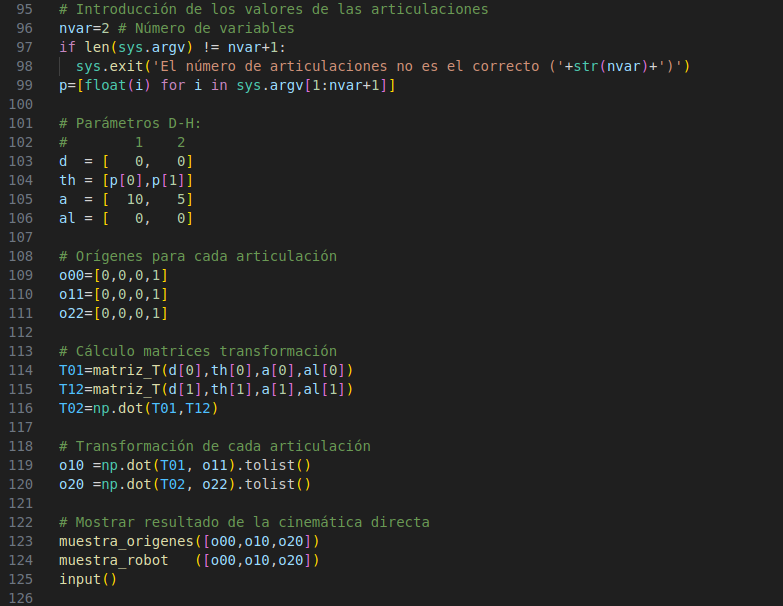
\includegraphics[width=1\linewidth]{images/cin_dir_1.png}
   \caption{Otra figura}
   \label{chapter:cap3}
\end{figure}
%%%%%%%%%%%%%%%%%%%%%%%%%%%%%%%%%%%%%%%%%%%%%%%%%%%%%%%%%%%%%
\section{Ejercicios}
Se proponen 4 manipuladores para los que se debe calcular la cinemática directa. Como se proporciona la solución del primero a modo de ejemplo, en este apartado se incluyen las soluciones de los ejercicios 2, 3 y 4.
\subsection{Manipulador 2}
\subsection{Manipulador 3}
\subsection{Manipulador 4}

\section{Mejoras}
En primer lugar, se abordan las mejoras implementadas.
\subsection{Apartado Uno}

A continuación, se describen las mejoras propuestas, que no se han llegado a implementar.


\section{Conclusions}